\section{Contribution}

\section{Rail}
\label{rail}
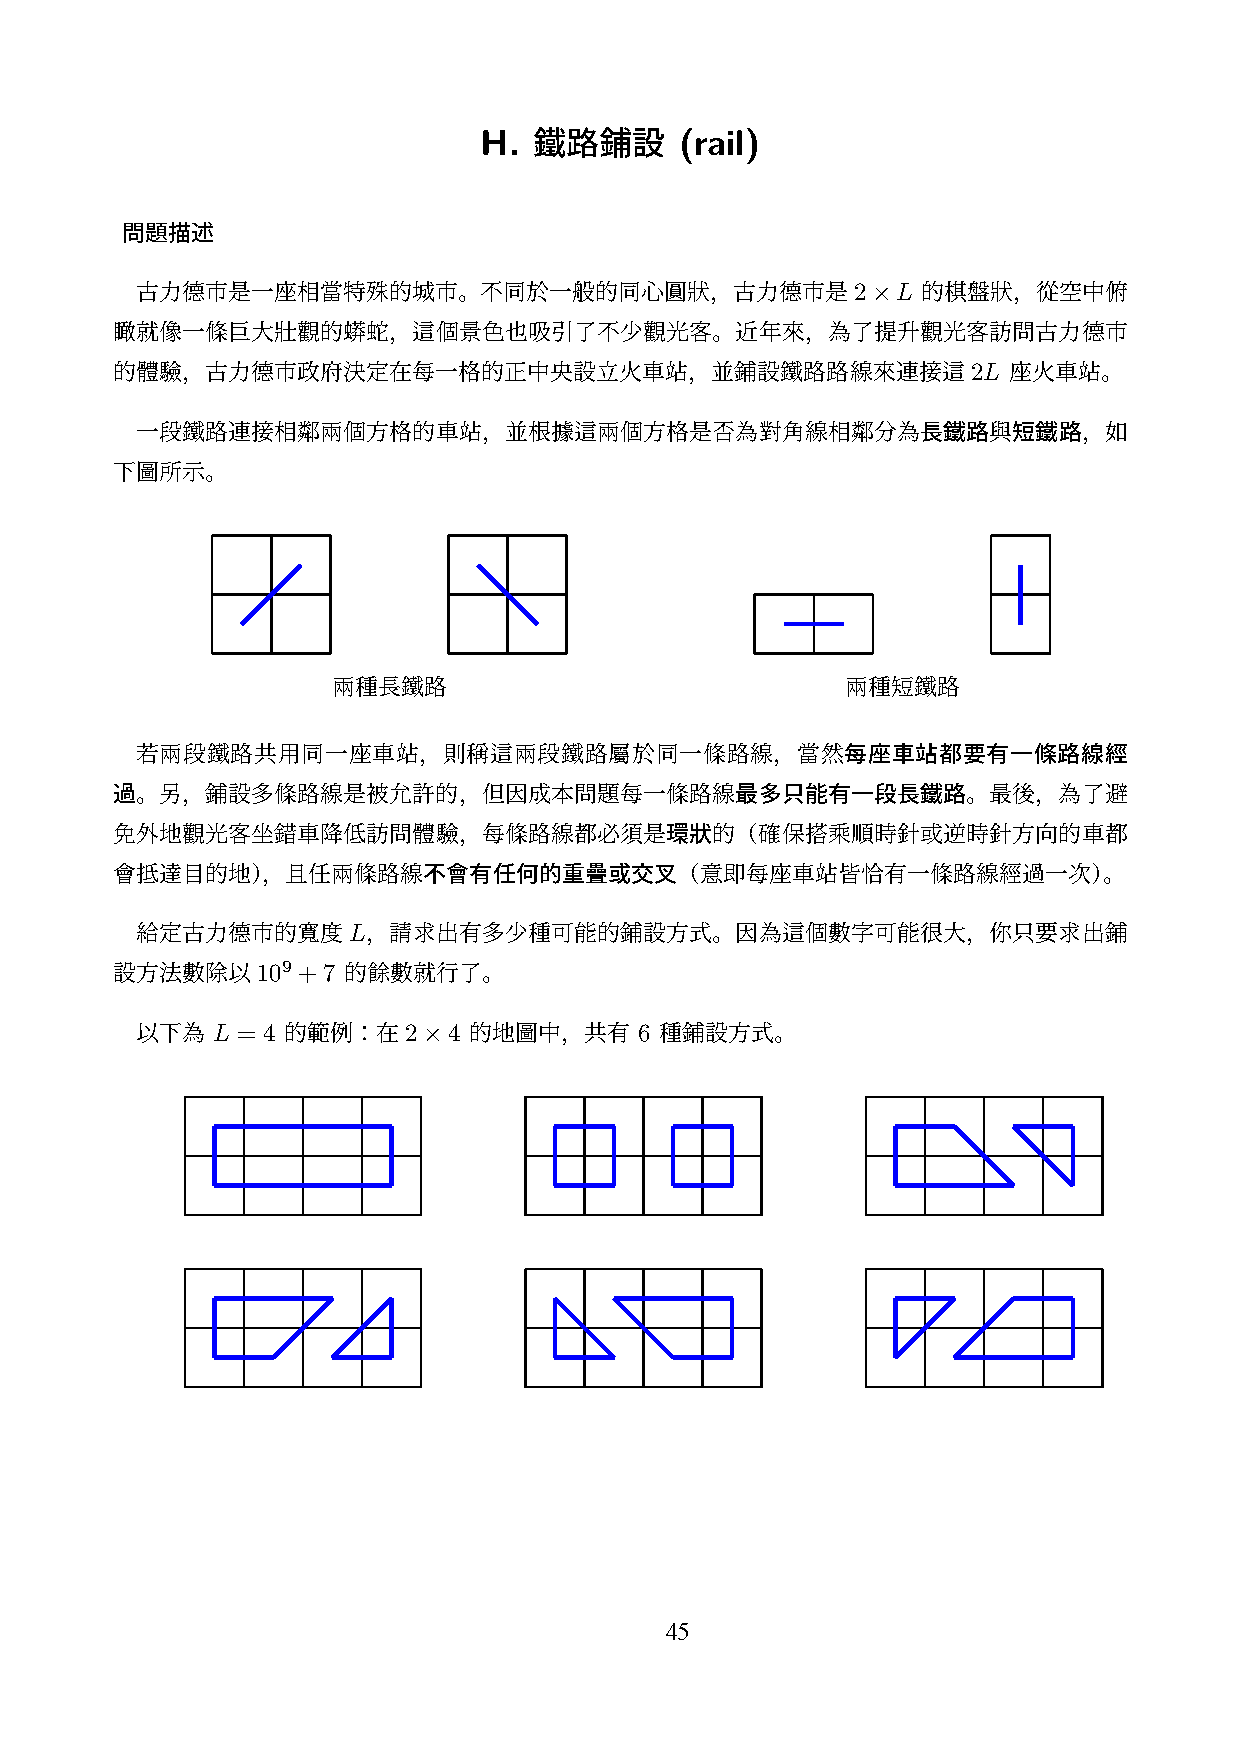
\includepdf[pages=-]{appendices/rail.pdf}

\section{Induction for the Transition Matrix of Rail}
\label{induction for Rail}

\subsection{Induction to recursive formula} 

\section{Code for Fibonacci}
\label{Fibonacci Code}
\subsection{Using Recursion}
\lstinputlisting[language=C++]{appendices/fibonacci_recursion.cpp}

\subsection{Using DP}
\lstinputlisting[language=C++]{appendices/fibonacci.cpp}

\subsection{Using Fast Matrix Power}
\lstinputlisting[language=C++]{appendices/fibonacci_bignum_2.cpp}

\section{Code for Rail}
\label{Rail Code}
\subsection{Using Recursion}
\lstinputlisting[language=C++]{appendices/rail_recursion.cpp}
\subsection{Using DP}
\lstinputlisting[language=C++]{appendices/rail.cpp}
\subsection{Using Fast Matrix Power}
\lstinputlisting[language=C++]{appendices/rail_bignum.cpp}



\begin{equation}
    D_i = \sum\limits_{j = c_1}^{n - c_2}(an + c_3)D_j + b \sum\limits_{j = c_1}^{n - c_2} j D_j
\end{equation}